\chapter{Dizajn i implementacija sustava}
\label{ch:system_design_implementation}

\selectlanguage{croatian}

\section{Korištene tehnologije}

Ključne tehnologije korištene u implementaciji uključuju ChromaDB kao vektorsku bazu podataka za pohranu i pretraživanje semantičkih ugradbi, Sentence Transformers modele za generiranje visokokvalitetnih vektorskih reprezentacija teksta, i OpenAI GPT-4 model za generiranje SPARQL upita iz prirodnog jezika.

\begin{figure}[h!]
    \centering
    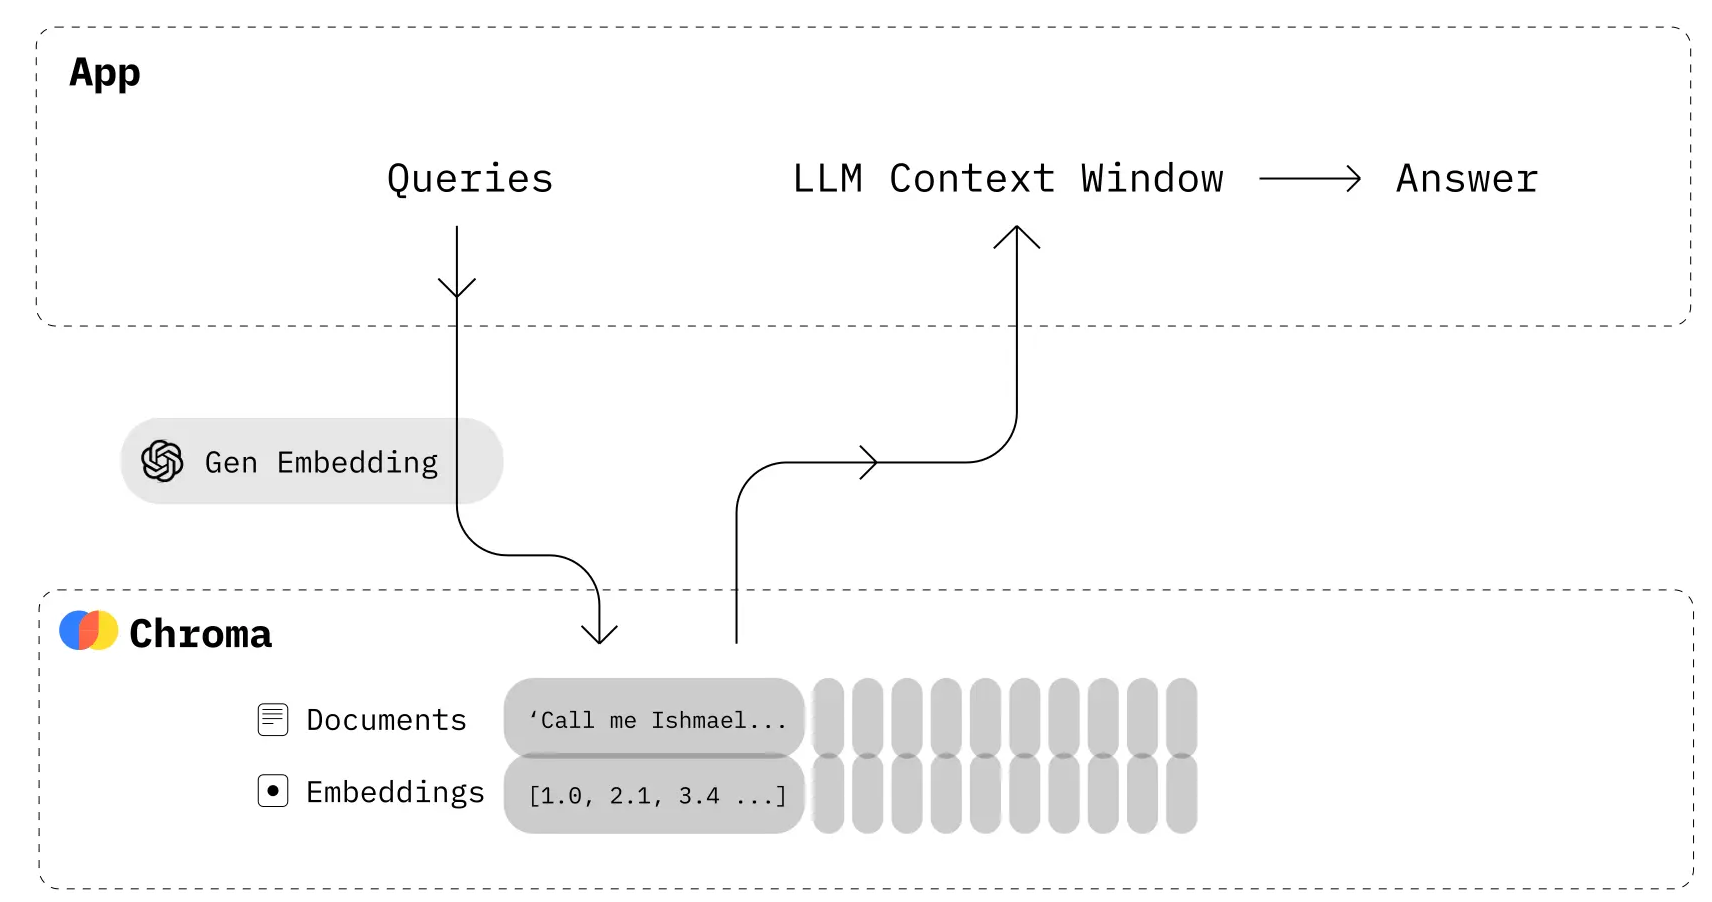
\includegraphics[width=1\textwidth]{figures/chroma.png}
    \caption{ChromaDB arhitektura - prikazuje komponente vektorske baze podataka}
    \label{fig:chromadb_architecture}
\end{figure}

LangChain okvir korišten je za orkestraciju različitih komponenti sustava i upravljanje agentima koji omogućavaju složene zadatke poput multimodalnog pretraživanja i inteligentne sinteze rezultata. Ova arhitektura omogućava modularnost i proširivost sustava.

\section{Ključne funkcionalnosti}

Automatska ekstrakcija sheme iz SPARQL endpointa omogućava dinamičko prilagođavanje sustava promjenama u strukturi podataka. Ova funkcionalnost je ključna za održavanje točnosti generiranih upita i omogućava sustavu da radi s različitim portalima otvorenih podataka.

\begin{figure}[htbp]
    \centering
    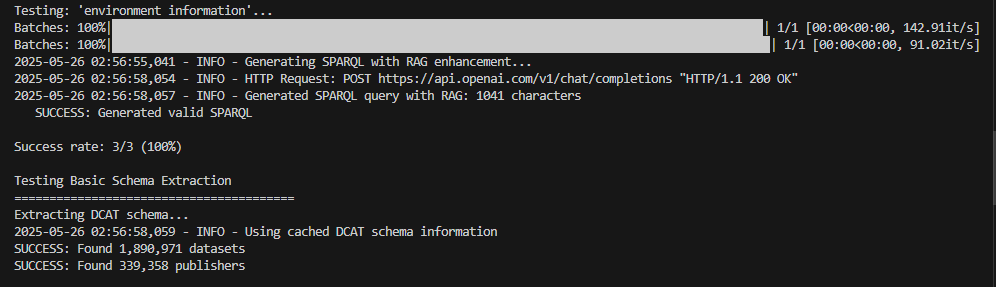
\includegraphics[width=1\textwidth]{figures/izvjestaj_image_11.png}
    \caption{Ekstrakcija sheme i validacija generiranog SPARQL upita}
    \label{fig:schema_extraction}
\end{figure}

Validacija upita implementirana je kroz dvostupanjski proces koji uključuje sintaksnu i semantičku provjeru. Ovo osigurava da se ne izvršavaju neispravni upiti koji mogu uzrokovati probleme s performansama ili pogrešne rezultate.

Multimodalni pristup pretraživanju omogućava kombiniranje različitih strategija za sveobuhvatno otkrivanje skupova podataka. Ovo uključuje RAG-prošireno SPARQL pretraživanje, REST API pozive i pronalaženje sličnih skupova podataka.

\begin{figure}[htbp]
    \centering
    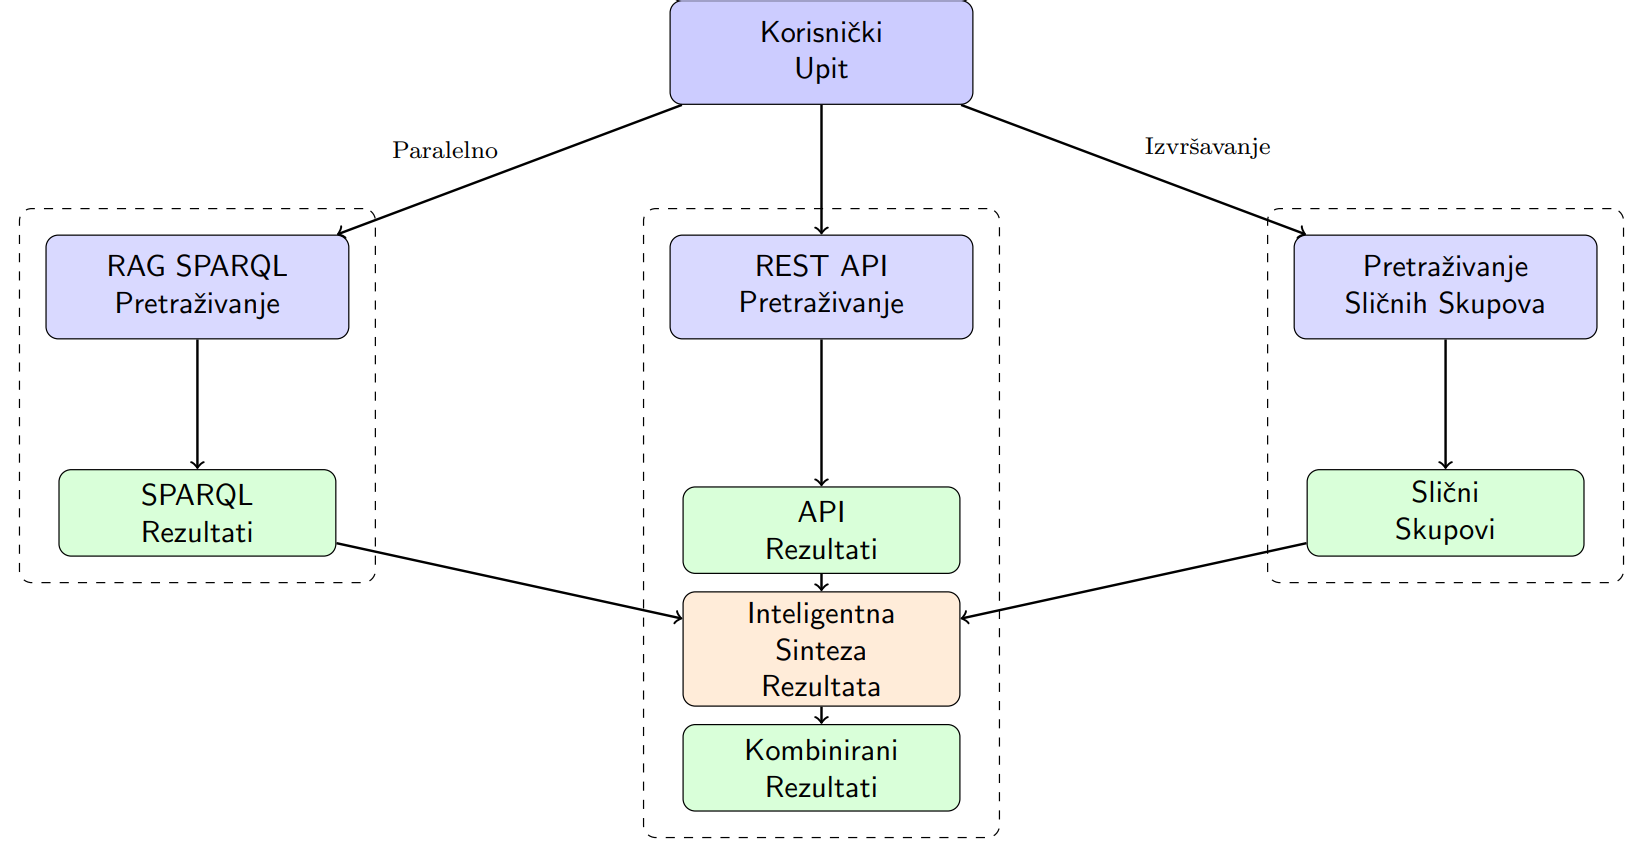
\includegraphics[width=1\textwidth]{figures/multimodal_search.png}
    \caption{Multimodalno pretraživanje - prikazuje različite strategije i njihovu integraciju}
    \label{fig:multimodal_search}
\end{figure}

\section{Arhitektura i skalabilnost}

Sustav je dizajniran da bude skalabilan i održiv, s jasno definiranim sučeljima između komponenti i robusnim mehanizmima rukovanja greškama. Ova arhitektura omogućava lako proširivanje i prilagodbu drugim portalima otvorenih podataka.

\begin{figure}[htbp]
    \centering
    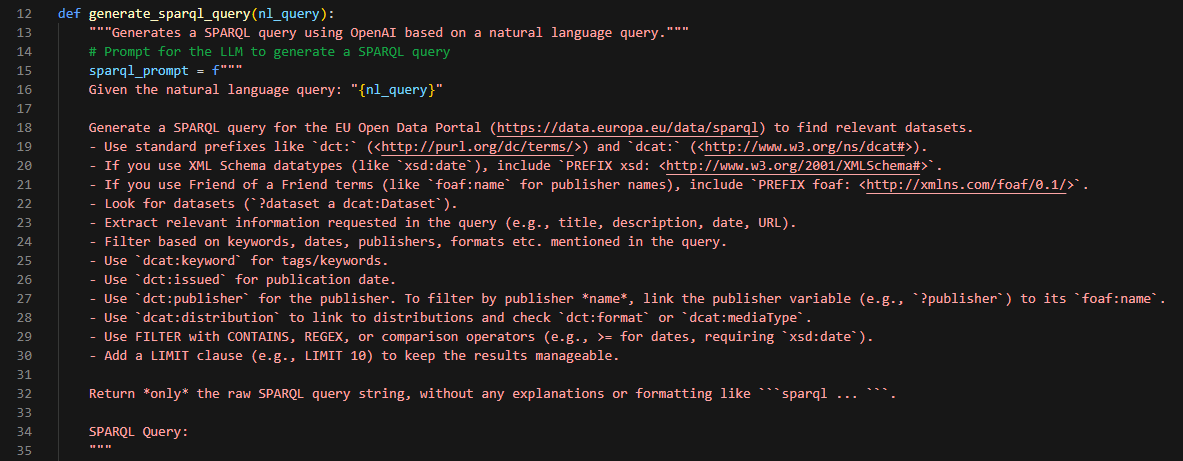
\includegraphics[width=1\textwidth]{figures/izvjestaj_image_13.png}
    \caption{Skalabilnost sustava - prikazuje mogućnosti proširivanja i optimizacije}
    \label{fig:system_scalability}
\end{figure}

Evaluacija korisničkog iskustva pokazuje da sustav pruža intuitivno sučelje koje omogućava korisnicima bez tehničke pozadine da učinkovito otkrivaju i analiziraju skupove podataka. Ovo demokratizira pristup otvorenim podacima i omogućava širu primjenu u različitim domenama.

\begin{figure}[htbp]
    \centering
    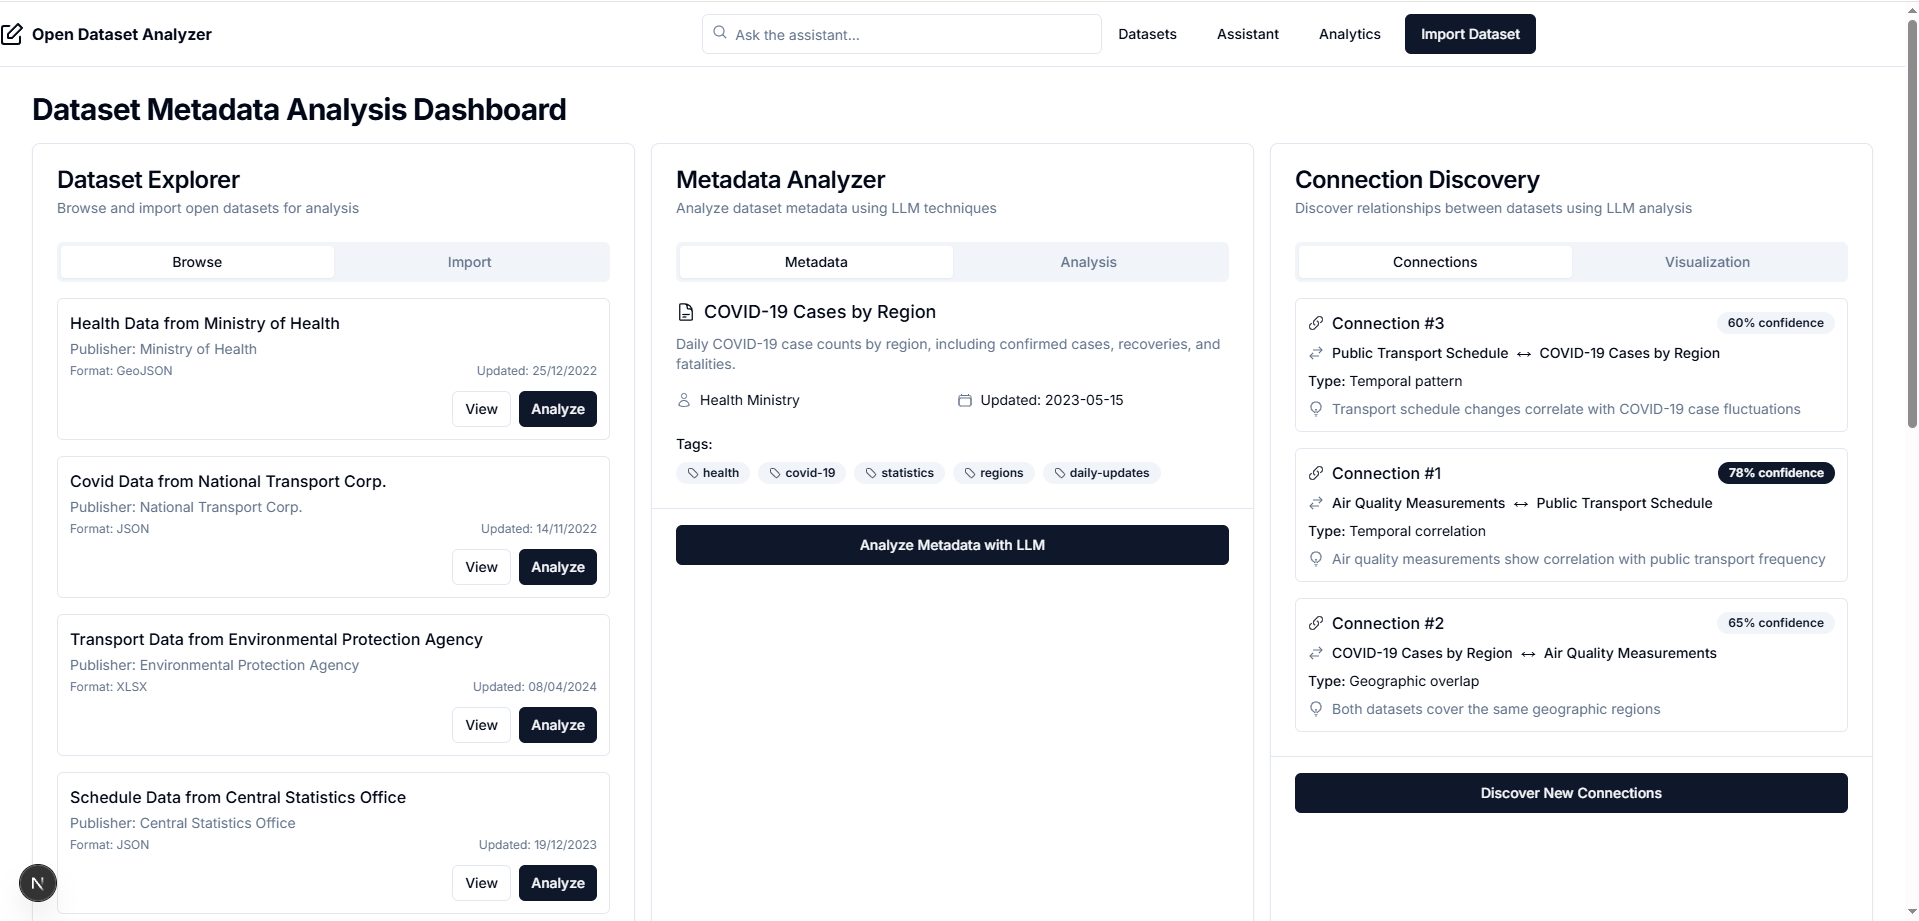
\includegraphics[width=1\textwidth]{figures/izvjestaj_image_4.png}
    \caption{Korisničko sučelje - prikazuje intuitivan dizajn i funkcionalnosti}
    \label{fig:user_interface}
\end{figure}

Sustav je dizajniran kao modularna arhitektura s jasno definiranim sučeljima između komponenti. Glavni razlog za ovakav pristup je mogućnost nezavisnog razvoja i testiranja pojedinačnih dijelova, što se pokazalo ključnim tijekom implementacije kada je bilo potrebno ispravljati probleme s vektorskim pretraživanjem ili optimizirati LLM pozive.

Arhitektura se sastoji od tri glavna sloja. Sloj pohrane koristi ChromaDB~\cite{wang2023vector} kao vektorsku bazu podataka za pohranu i pretraživanje semantičkih ugradbi, Sentence Transformers modele~\cite{reimers2019sentence} za generiranje visokokvalitetnih vektorskih reprezentacija teksta, i OpenAI GPT-4 model~\cite{brown2020language} za generiranje SPARQL upita iz prirodnog jezika. ChromaDB omogućava brzo pretraživanje sličnosti (kosinusna sličnost) i podržava pohranu meta podataka, što je bilo važno za spremanje informacija o SPARQL upitima i shemi. U praksi se pokazalo da ChromaDB može učinkovito rukovati s velikim brojem primjera upita bez značajnih problema s performansama.

Sloj obrade uključuje Sentence Transformers model all-MiniLM-L6-v2 za generiranje embeddinga. Ovaj model je odabran nakon testiranja nekoliko alternativa - pokazao se kao optimalan balans između kvalitete embeddinga, brzine generiranja i veličine modela. Model generira 384-dimenzijske vektore što je dovoljno za hvatanje semantičkih razlika, a dovoljno malo za brzo pretraživanje. Testiranje je pokazalo da model dobro radi s hrvatskim i engleskim tekstom, što je bilo važno za podatke s EU Portala.

LangChain okvir~\cite{liu2023survey} korišten je za orkestraciju različitih komponenti sustava i upravljanje agentima koji omogućavaju složene zadatke poput multimodalnog pretraživanja i inteligentne sinteze rezultata.

OpenAI GPT-4 je korišten za generiranje SPARQL upita. Model pokazuje izvrsne rezultate kada ima dovoljno kontekstualnih informacija, ali ima ograničenja s tokenima što može biti problematično za složene upite. Također, troškovi API poziva mogu biti značajni za intenzivnu upotrebu.

\begin{figure}[htbp]
    \centering
    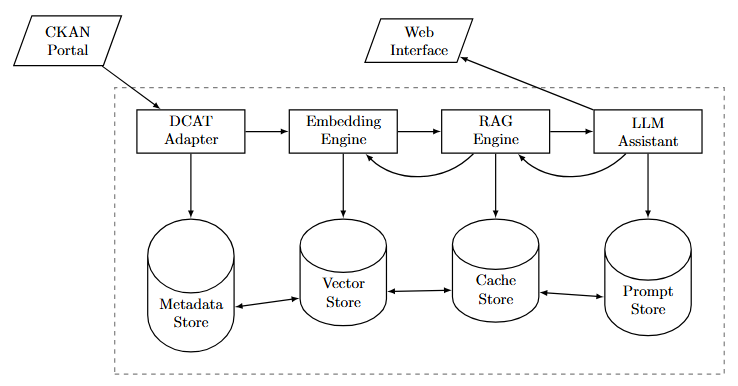
\includegraphics[width=1\textwidth]{figures/system_architecture.png}
    \caption{Arhitektura sustava - prikazuje tok podataka kroz različite komponente}
    \label{fig:system_architecture}
\end{figure}

\section{Implementacija RAG sustava i vektorske baze}

RAG sustav~\cite{lewis2020retrieval} je implementiran u src/rag\_system.py i predstavlja srce cijelog sustava. Glavna klasa RAGSystem upravlja svim aspektima RAG pipeline-a od generiranja embeddinga do izvršavanja upita.

Inicijalizacija sustava uključuje postavljanje ChromaDB klijenta, učitavanje Sentence Transformers modela i konfiguraciju OpenAI klijenta. ChromaDB koristi trajno pohranjivanje što omogućava da se embeddingi sačuvaju između pokretanja sustava. Ovo je bilo ključno za performanse jer generiranje embeddinga može biti sporo, posebno za velike kolekcije teksta.

Generiranje embeddinga se vrši kroz metodu generate\_embedding koja koristi Sentence Transformers model. Implementacija uključuje caching mehanizam koji sprečava ponovno generiranje embeddinga za iste tekstove. Caching je implementiran kao jednostavan dictionary u memoriji, ali za produkcijsku upotrebu bi trebao biti implementiran kao Redis ili sličan sustav.

Dodavanje primjera upita u vektorsku bazu se vrši kroz metodu add\_query\_example. Svaki primjer se sastoji od pitanja na prirodnom jeziku, odgovarajućeg SPARQL upita, opisa i tagova. Embedding se generira za pitanje, a metadata se sprema zajedno s embeddingom. Ovo omogućava kasnije pretraživanje sličnih primjera na temelju semantičke sličnosti.

\begin{lstlisting}[language=Python, caption=Implementacija dodavanja primjera u vektorsku bazu]
def add_query_example(self, example: QueryExample) -> str:
    """Dodaj primjer pitanje-upit par u vektorsku bazu"""
    
    # Provjeri cache za embedding
    cache_key = f"embedding_{hash(example.question)}"
    if cache_key in self.embedding_cache:
        embedding = self.embedding_cache[cache_key]
    else:
        embedding = self._generate_embedding(example.question)
        self.embedding_cache[cache_key] = embedding
    
    # Generiraj jedinstveni ID
    doc_id = f"example_{len(self.query_examples_collection.get()['ids'])}"
    
    # Spremi u ChromaDB
    self.query_examples_collection.add(
        documents=[example.question],
        embeddings=[embedding],
        metadatas=[{
            "sparql_query": example.sparql_query,
            "endpoint": example.endpoint,
            "description": example.description,
            "tags": json.dumps(example.tags),
            "added_at": datetime.now().isoformat(),
            "success_rate": example.success_rate if hasattr(example, 'success_rate') else None
        }],
        ids=[doc_id]
    )
    
    return doc_id
\end{lstlisting}

Semantička pretraga sličnih primjera je implementirana kroz metodu retrieve\_similar\_examples. Metoda koristi kosinusnu sličnost za pronalaženje najsličnijih primjera u vektorskom prostoru. Implementacija uključuje opciju za filtriranje rezultata na temelju tagova ili endpointa, što može biti korisno za specifične domene.

\begin{lstlisting}[language=Python, caption=Implementacija semantičke pretrage]
def retrieve_similar_examples(self, query: str, n_results: int = 5, filters: Dict = None) -> List[Dict[str, Any]]:
    """Dohvati slične primjere koristeći vektorsku pretragu"""
    
    # Generiraj ugradbu za upit
    query_embedding = self._generate_embedding(query)
    
    # Postavi filtere ako su zadani
    where_clause = None
    if filters:
        where_clause = {}
        if 'tags' in filters:
            where_clause['tags'] = {'$contains': filters['tags']}
        if 'endpoint' in filters:
            where_clause['endpoint'] = filters['endpoint']
    
    # Izvedi vektorsku pretragu
    results = self.query_examples_collection.query(
        query_embeddings=[query_embedding],
        n_results=n_results,
        where=where_clause
    )
    
    # Obradi rezultate
    similar_examples = []
    if results['documents'] and results['documents'][0]:
        for i, doc in enumerate(results['documents'][0]):
            metadata = results['metadatas'][0][i]
            similar_examples.append({
                "question": doc,
                "sparql_query": metadata.get("sparql_query"),
                "distance": results['distances'][0][i],
                "success_rate": metadata.get("success_rate"),
                "tags": json.loads(metadata.get("tags", "[]"))
            })
    
    return similar_examples
\end{lstlisting}

\begin{figure}[h!]
    \centering
    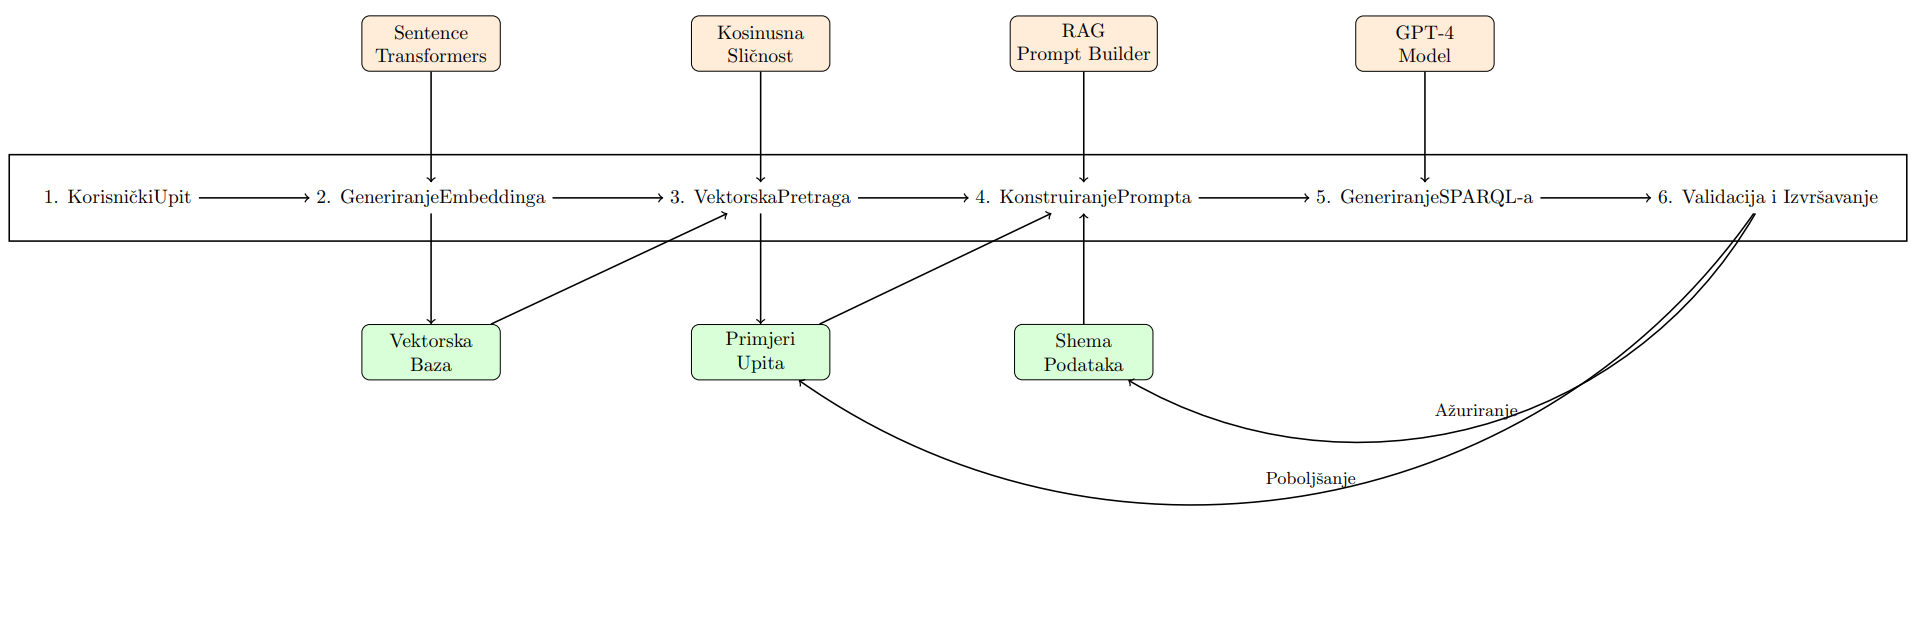
\includegraphics[width=1\textwidth]{figures/rag_pipeline.png}
    \caption{RAG pipeline - prikazuje tok od upita do generiranog SPARQL-a}
    \label{fig:rag_pipeline}
\end{figure}

\section{Generiranje SPARQL upita i prompt engineering}

Generiranje SPARQL upita iz prirodnog jezika je najsloženiji dio sustava. Implementacija koristi RAG pristup gdje se korisnički upit proširuje s relevantnim primjerima i informacijama o shemi prije slanja LLM-u.

Konstruiranje prompta se vrši kroz metodu build\_rag\_prompt koja kombinira korisnički upit s dohvaćenim primjerima i informacijama o shemi. Prompt je strukturiran u nekoliko sekcija: kontekst upita, slični primjeri, informacije o shemi i instrukcije za generiranje. Ova struktura se pokazala kao ključna za kvalitetu generiranih upita.

\begin{lstlisting}[language=Python, caption=Implementacija konstruiranja RAG prompta]
def build_rag_prompt(self, user_query: str, context: str = "") -> str:
    """Konstruiraj poboljšani prompt koristeći RAG tehnologiju"""
    
    # Dohvati slične primjere i informacije o shemi
    similar_examples = self.retrieve_similar_examples(user_query, n_results=3)
    schema_info = self.retrieve_relevant_schema(user_query, n_results=2)
    
    # Počni s osnovnim promptom
    prompt = f"""You are an expert SPARQL query generator for the EU Open Data Portal.
    
User Query: "{user_query}"
{f"Additional Context: {context}" if context else ""}

Your task is to generate a valid SPARQL query that retrieves the requested data.
Use the following examples and schema information as guidance.

## Similar Query Examples:
"""
    
    # Dodaj slične primjere
    for i, example in enumerate(similar_examples):
        prompt += f"""
Example {i+1}:
Question: {example['question']}
SPARQL Query:
{example['sparql_query']}
Distance: {example['distance']:.3f}
"""
    
    # Dodaj informacije o shemi
    if schema_info:
        prompt += "\n## Available Schema Information:\n"
        for i, schema in enumerate(schema_info):
            prompt += f"""
Schema {i+1}:
Classes: {', '.join([cls.get('name', '') for cls in schema['classes'][:10]])}
Properties: {', '.join([prop.get('name', '') for prop in schema['properties'][:15]])}
"""
    
    # Dodaj instrukcije
    prompt += """
## Instructions:
1. Generate a valid SPARQL query that matches the user's intent
2. Use appropriate prefixes (dcat:, dct:, foaf:, etc.)
3. Include proper WHERE clauses and OPTIONAL patterns where needed
4. Limit results to reasonable number (e.g., LIMIT 100)
5. Return only the SPARQL query, no explanations

SPARQL Query:
"""
    
    return prompt
\end{lstlisting}

Generiranje upita se vrši kroz metodu generate\_sparql\_query koja koristi OpenAI GPT-4 model. Implementacija uključuje error handling i retry logiku za slučaj API grešaka. Također, implementiran je mehanizam za validaciju generiranih upita prije izvršavanja.

\begin{lstlisting}[language=Python, caption=Implementacija generiranja SPARQL upita]
def generate_sparql_query(self, user_query: str, context: str = "") -> Dict[str, Any]:
    """Generiraj SPARQL upit iz prirodnog jezika"""
    
    try:
        # Konstruiraj prompt
        prompt = self.build_rag_prompt(user_query, context)
        
        # Pozovi LLM
        response = self.llm.invoke(prompt)
        
        # Ekstraktiraj SPARQL upit iz odgovora
        sparql_query = self._extract_sparql_from_response(response.content)
        
        # Validiraj upit
        validation_result = self.validate_sparql_query(sparql_query)
        
        return {
            "sparql_query": sparql_query,
            "is_valid": validation_result["is_valid"],
            "errors": validation_result.get("errors", []),
            "warnings": validation_result.get("warnings", []),
            "prompt_used": prompt,
            "model_response": response.content
        }
        
    except Exception as e:
        return {
            "sparql_query": None,
            "is_valid": False,
            "errors": [str(e)],
            "prompt_used": prompt if 'prompt' in locals() else None
        }
\end{lstlisting}

\begin{figure}[htbp]
    \centering
    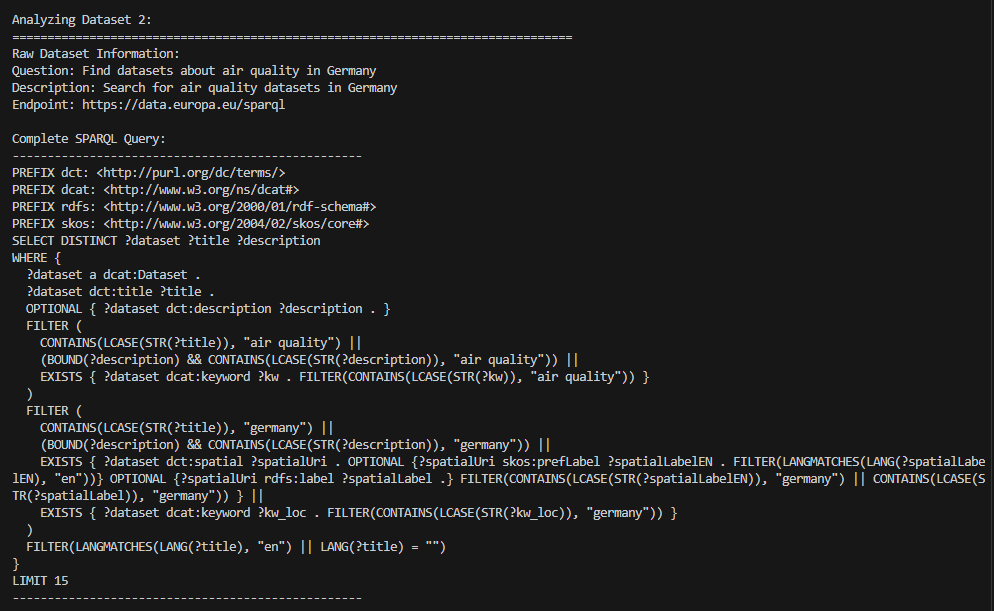
\includegraphics[width=1\textwidth]{figures/izvjestaj_image_53.png}
    \caption{Generiranje SPARQL upita}
    \label{fig:unified_data_assistant}
\end{figure}

Validacija upita je implementirana kroz dvostupanjski proces. Prvi korak je sintaksna validacija kroz SPARQL parser, a drugi korak je testiranje izvršavanja s ograničenim brojem rezultata. Ovo sprečava izvršavanje neispravnih upita koji mogu uzrokovati probleme s performansama.

\begin{figure}[htbp]
    \centering
    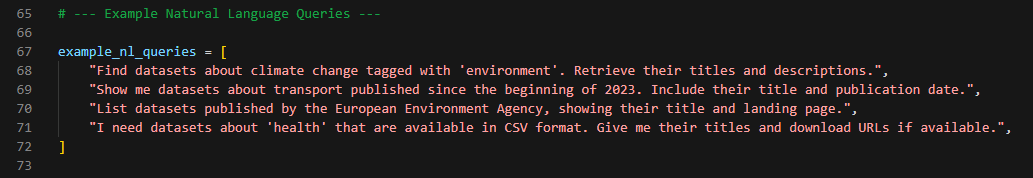
\includegraphics[width=1\textwidth]{figures/izvjestaj_image_84.png}
    \caption{Primjer prompta - struktura i elementi prompta za LLM}
    \label{fig:prompt_example}
\end{figure}

\section{Ekstrakcija sheme i DCAT analiza}

Automatska ekstrakcija sheme iz SPARQL endpointa je ključna komponenta sustava koja omogućava dinamičko prilagođavanje promjenama u strukturi podataka. Implementacija je specifično prilagođena za EU Portal otvorenih podataka i DCAT metapodatke.

VoID deskriptor ekstrakcija se vrši kroz SPARQL upite koji dohvaćaju informacije o strukturi grafa znanja. Implementacija uključuje dohvaćanje broja trojki, različitih subjekata, klasa i svojstava. Ove informacije su ključne za razumijevanje strukture podataka i optimizaciju upita.

\begin{lstlisting}[language=Python, caption=Implementacija VoID deskriptor ekstrakcije]
def get_void_description(self) -> Dict[str, Any]:
    """Ekstraktiraj VoID opis grafa znanja"""
    
    void_query = """
    PREFIX void: <http://rdfs.org/ns/void#>
    PREFIX dct: <http://purl.org/dc/terms/>
    PREFIX foaf: <http://xmlns.com/foaf/0.1/>
    
    SELECT DISTINCT ?dataset ?title ?description ?subjects ?triples ?classes ?properties
    WHERE {
      ?dataset a void:Dataset .
      OPTIONAL { ?dataset dct:title ?title . }
      OPTIONAL { ?dataset dct:description ?description . }
      OPTIONAL { ?dataset void:distinctSubjects ?subjects . }
      OPTIONAL { ?dataset void:triples ?triples . }
      OPTIONAL { ?dataset void:classes ?classes . }
      OPTIONAL { ?dataset void:properties ?properties . }
    }
    LIMIT 10
    """
    
    try:
        results = self._execute_sparql_query(void_query)
        return self._process_void_results(results)
    except Exception as e:
        logger.error(f"Error extracting VoID description: {e}")
        return {}
\end{lstlisting}

DCAT analiza se fokusira na specifične aspekte EU Portala otvorenih podataka. Implementacija dohvaća informacije o skupovima podataka, distribucijama, izdavačima, temama i formatima. Ove informacije omogućavaju generiranje upita koji su optimizirani za specifične karakteristike EU Portala.

\begin{lstlisting}[language=Python, caption=Implementacija DCAT analize]
def analyze_dcat_structure(self) -> Dict[str, Any]:
    """Analiziraj DCAT strukturu grafa znanja"""
    
    dcat_queries = {
        "datasets": """
        PREFIX dcat: <http://www.w3.org/ns/dcat#>
        PREFIX dct: <http://purl.org/dc/terms/>
        
        SELECT ?dataset ?title ?publisher ?theme ?keyword
        WHERE {
          ?dataset a dcat:Dataset .
          OPTIONAL { ?dataset dct:title ?title . }
          OPTIONAL { ?dataset dct:publisher ?publisher . }
          OPTIONAL { ?dataset dcat:theme ?theme . }
          OPTIONAL { ?dataset dcat:keyword ?keyword . }
        }
        LIMIT 100
        """,
        
        "distributions": """
        PREFIX dcat: <http://www.w3.org/ns/dcat#>
        PREFIX dct: <http://purl.org/dc/terms/>
        
        SELECT ?dataset ?distribution ?format ?accessURL
        WHERE {
          ?dataset a dcat:Dataset .
          ?dataset dcat:distribution ?distribution .
          OPTIONAL { ?distribution dcat:mediaType ?format . }
          OPTIONAL { ?distribution dcat:accessURL ?accessURL . }
        }
        LIMIT 100
        """
    }
    
    results = {}
    for query_name, query in dcat_queries.items():
        try:
            results[query_name] = self._execute_sparql_query(query)
        except Exception as e:
            logger.error(f"Error in {query_name} analysis: {e}")
            results[query_name] = []
    
    return self._process_dcat_results(results)
\end{lstlisting}

Analiza klasa i svojstava omogućava razumijevanje najčešće korištenih pojmova u grafu znanja. Implementacija uključuje brojanje pojavljivanja različitih klasa i svojstava, što omogućava optimizaciju upita i generiranje relevantnih primjera.

\begin{lstlisting}[language=Python, caption=Implementacija analize klasa i svojstava]
def analyze_classes_and_properties(self) -> Dict[str, Any]:
    """Analiziraj klase i svojstva u grafu znanja"""
    
    class_query = """
    SELECT ?class (COUNT(?instance) as ?count)
    WHERE {
      ?instance a ?class .
    }
    GROUP BY ?class
    ORDER BY DESC(?count)
    LIMIT 50
    """
    
    property_query = """
    SELECT ?property (COUNT(?triple) as ?count)
    WHERE {
      ?s ?property ?o .
    }
    GROUP BY ?property
    ORDER BY DESC(?count)
    LIMIT 100
    """
    
    try:
        classes = self._execute_sparql_query(class_query)
        properties = self._execute_sparql_query(property_query)
        
        return {
            "classes": self._process_class_results(classes),
            "properties": self._process_property_results(properties)
        }
    except Exception as e:
        logger.error(f"Error analyzing classes and properties: {e}")
        return {"classes": [], "properties": []}
\end{lstlisting}

\section{Unified Data Assistant i multimodalno pretraživanje}

Unified Data Assistant predstavlja glavno sučelje sustava koje orkestrira različite strategije pretraživanja. Implementacija koristi LangChain agentski okvir za upravljanje složenim zadacima i omogućava multimodalno pretraživanje kroz SPARQL, REST API i similarity search.

Arhitektura agenta je dizajnirana da podržava različite tipove upita i automatski odabire najprikladniju strategiju pretraživanja. Implementacija uključuje alate za SPARQL pretraživanje, REST API pozive i pronalaženje sličnih skupova podataka.

\begin{lstlisting}[language=Python, caption=Implementacija Unified Data Assistant]
class UnifiedDataAssistant:
    def __init__(self, rag_system: RAGSystem, sparql_processor: SPARQLProcessor):
        self.rag_system = rag_system
        self.sparql_processor = sparql_processor
        self.llm = ChatOpenAI(model="gpt-4o", temperature=0.1)
        
        # Definiraj alate za agenta
        self.tools = [
            Tool(
                name="sparql_search",
                func=self._sparql_search,
                description="Pretraži podatke koristeći SPARQL upite"
            ),
            Tool(
                name="api_search",
                func=self._api_search,
                description="Pretraži podatke koristeći REST API"
            ),
            Tool(
                name="similar_datasets",
                func=self._similar_datasets,
                description="Pronađi slične skupove podataka"
            )
        ]
        
        # Inicijaliziraj agenta
        self.agent = initialize_agent(
            tools=self.tools,
            llm=self.llm,
            agent=AgentType.ZERO_SHOT_REACT_DESCRIPTION,
            verbose=True,
            max_iterations=5
        )
\end{lstlisting}

\begin{figure}[htbp]
    \centering
    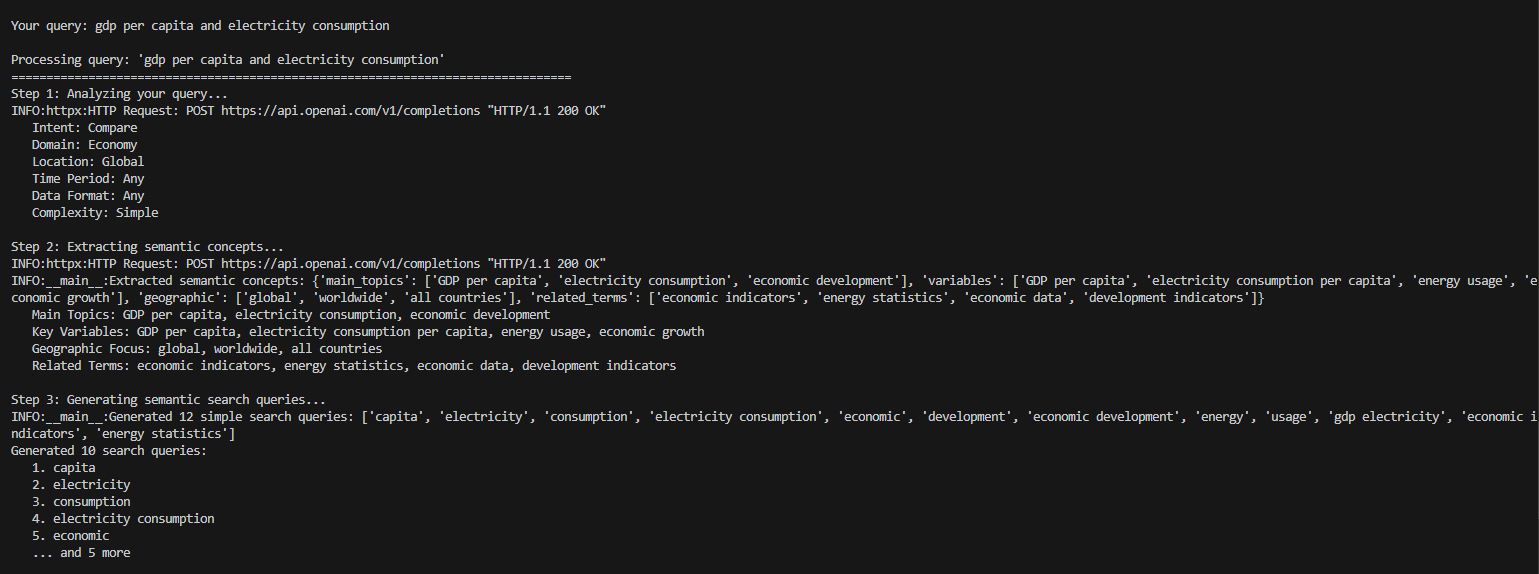
\includegraphics[width=1\textwidth]{figures/1.png}
    \caption{Pokretanje složenijeg upita}
    \label{fig:unified_data_assistant}
\end{figure}

Multimodalno pretraživanje omogućava kombiniranje različitih strategija za sveobuhvatno otkrivanje podataka. Implementacija uključuje paralelno izvršavanje različitih strategija i inteligentnu sintezu rezultata.

\begin{lstlisting}[language=Python, caption=Implementacija multimodalnog pretraživanja]
def search_datasets(self, query: str) -> Dict[str, Any]:
    """Izvedi multimodalno pretraživanje skupova podataka"""
    
    results = {
        "sparql_results": [],
        "api_results": [],
        "similar_datasets": [],
        "combined_analysis": "",
        "errors": []
    }
    
    # 1. RAG-prošireno SPARQL pretraživanje
    try:
        sparql_query = self.rag_system.generate_sparql_query(query)
        if sparql_query.get("is_valid"):
            results["sparql_results"] = self.sparql_processor.execute_query(
                sparql_query["sparql_query"]
            )
        else:
            results["errors"].append(f"SPARQL generation failed: {sparql_query.get('errors')}")
    except Exception as e:
        results["errors"].append(f"SPARQL search error: {str(e)}")
    
    # 2. REST API pretraživanje
    try:
        results["api_results"] = self._search_api(query)
    except Exception as e:
        results["errors"].append(f"API search error: {str(e)}")
    
    # 3. Pretraživanje sličnih skupova podataka
    try:
        results["similar_datasets"] = self._find_similar_datasets(query)
    except Exception as e:
        results["errors"].append(f"Similar datasets error: {str(e)}")
    
    # 4. Inteligentna sinteza rezultata
    try:
        results["combined_analysis"] = self._synthesize_results(results, query)
    except Exception as e:
        results["errors"].append(f"Synthesis error: {str(e)}")
    
    return results
\end{lstlisting}

\begin{figure}[htbp]
    \centering
    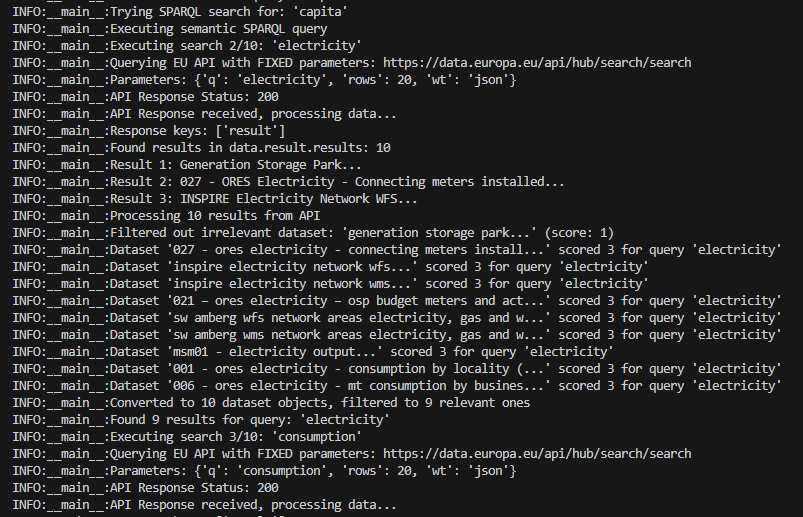
\includegraphics[width=1\textwidth]{figures/2.png}
    \caption{Multimodalno pretraživanje}
    \label{fig:unified_data_assistant}
\end{figure}

Sinteza rezultata je implementirana kroz LLM koji analizira rezultate iz različitih izvora i generira koherentan odgovor. Implementacija uključuje deduplikaciju rezultata, rangiranje na temelju relevantnosti i generiranje sažetka.

\begin{lstlisting}[language=Python, caption=Implementacija sinteze rezultata]
def _synthesize_results(self, results: Dict[str, Any], original_query: str) -> str:
    """Sintetiziraj rezultate iz različitih izvora"""
    
    # Pripremi podatke za sintezu
    synthesis_data = {
        "original_query": original_query,
        "sparql_count": len(results.get("sparql_results", [])),
        "api_count": len(results.get("api_results", [])),
        "similar_count": len(results.get("similar_datasets", [])),
        "errors": results.get("errors", [])
    }
    
    # Dodaj primjere rezultata
    if results.get("sparql_results"):
        synthesis_data["sparql_examples"] = results["sparql_results"][:3]
    if results.get("api_results"):
        synthesis_data["api_examples"] = results["api_results"][:3]
    if results.get("similar_datasets"):
        synthesis_data["similar_examples"] = results["similar_datasets"][:3]
    
    # Konstruiraj prompt za sintezu
    synthesis_prompt = f"""
    Analyze the following search results for the query: "{original_query}"
    
    Results Summary:
    - SPARQL results: {synthesis_data['sparql_count']} items
    - API results: {synthesis_data['api_count']} items  
    - Similar datasets: {synthesis_data['similar_count']} items
    - Errors: {len(synthesis_data['errors'])}
    
    Provide a comprehensive analysis that:
    1. Summarizes the main findings
    2. Identifies the most relevant datasets
    3. Suggests next steps for the user
    4. Notes any limitations or issues encountered
    
    Focus on practical insights and actionable information.
    """
    
    try:
        response = self.llm.invoke(synthesis_prompt)
        return response.content
    except Exception as e:
        return f"Error synthesizing results: {str(e)}"
\end{lstlisting}

\begin{figure}[htbp]
    \centering
    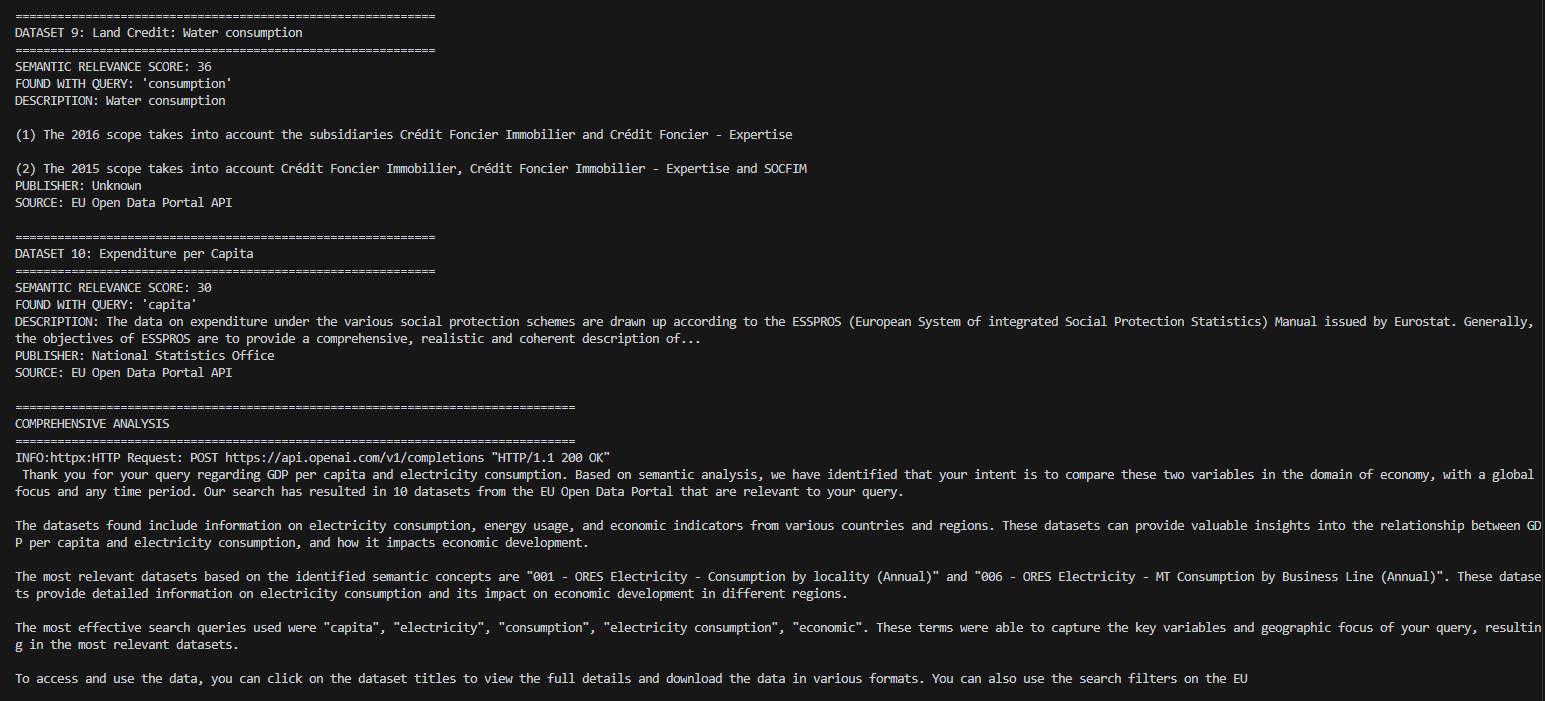
\includegraphics[width=1\textwidth]{figures/ranking_combined_results2.png}
    \caption{Rangiranje kombiniranih rezultata}
    \label{fig:unified_data_assistant}
\end{figure}

\section{Validacija, rukovanje greškama i optimizacija}

Robusno rukovanje greškama je ključno za pouzdano funkcioniranje sustava. Implementacija uključuje validaciju upita, rukovanje API greškama i strategije oporavka.

Validacija SPARQL upita se vrši kroz dvostupanjski proces. Prvi korak je sintaksna validacija kroz SPARQL parser, a drugi korak je testiranje izvršavanja s ograničenim brojem rezultata. Ovo sprječava izvršavanje neispravnih upita koji mogu uzrokovati probleme s performansama.

\begin{lstlisting}[language=Python, caption=Implementacija validacije SPARQL upita]
def validate_sparql_query(self, query: str) -> Dict[str, Any]:
    """Validiraj SPARQL upit"""
    
    validation_result = {
        "is_valid": False,
        "syntax_errors": [],
        "semantic_errors": [],
        "warnings": [],
        "execution_time": None
    }
    
    # Provjeri sintaksu
    try:
        parsed_query = parse_sparql_query(query)
        validation_result["is_valid"] = True
    except Exception as e:
        validation_result["syntax_errors"].append(str(e))
        return validation_result
    
    # Provjeri semantiku kroz test izvršavanja
    try:
        start_time = time.time()
        test_query = query.replace("LIMIT", "LIMIT 1")
        test_results = self._execute_sparql_query(test_query)
        execution_time = time.time() - start_time
        
        validation_result["execution_time"] = execution_time
        
        if test_results is None or len(test_results) == 0:
            validation_result["warnings"].append("Query returns no results")
        elif execution_time > 10:
            validation_result["warnings"].append("Query may be slow")
            
    except Exception as e:
        validation_result["semantic_errors"].append(str(e))
        validation_result["is_valid"] = False
    
    return validation_result
\end{lstlisting}

Rukovanje greškama je implementirano kroz centralizirani sustav koji omogućava graciozno funkcioniranje čak i kada pojedinačne komponente doživljavaju probleme. Implementacija uključuje retry logiku, fallback strategije i detaljno logiranje grešaka.

\begin{lstlisting}[language=Python, caption=Implementacija rukovanja greškama]
def handle_errors(self, error: Exception, context: str) -> Dict[str, Any]:
    """Rukuj greškama na elegantan način"""
    
    error_response = {
        "error_type": type(error).__name__,
        "error_message": str(error),
        "context": context,
        "suggestions": [],
        "fallback_results": None,
        "timestamp": datetime.now().isoformat()
    }
    
    # Dodaj prijedloge za rješavanje na temelju tipa greške
    if "timeout" in str(error).lower():
        error_response["suggestions"].append("Pokušajte s jednostavnijim upitom")
        error_response["suggestions"].append("Provjerite mrežnu vezu")
    elif "syntax" in str(error).lower():
        error_response["suggestions"].append("Provjerite sintaksu upita")
        error_response["suggestions"].append("Koristite jednostavniji jezik")
    elif "rate limit" in str(error).lower():
        error_response["suggestions"].append("Pričekajte prije novog pokušaja")
        error_response["suggestions"].append("Smanjite broj istovremenih zahtjeva")
    
    # Pokušaj fallback strategiju
    try:
        error_response["fallback_results"] = self._fallback_search(context)
    except Exception as fallback_error:
        error_response["fallback_error"] = str(fallback_error)
    
    # Logiraj grešku
    logger.error(f"Error in {context}: {error}")
    
    return error_response
\end{lstlisting}

Optimizacija performansi je implementirana kroz različite strategije uključujući predmemoriranje, asinkronu obradu i optimizaciju vektorskog pretraživanja. Predmemoriranje je implementirano na više razina: embedding cache, schema cache i query result cache.

\begin{lstlisting}[language=Python, caption=Implementacija predmemoriranja]
class CacheManager:
    def __init__(self, max_size: int = 1000):
        self.embedding_cache = {}
        self.schema_cache = {}
        self.query_cache = {}
        self.max_size = max_size
    
    def get_cached_embedding(self, text: str) -> Optional[List[float]]:
        """Dohvati predmemoriranu ugradbu"""
        return self.embedding_cache.get(text)
    
    def cache_embedding(self, text: str, embedding: List[float]):
        """Predmemoriraj ugradbu"""
        if len(self.embedding_cache) >= self.max_size:
            # Ukloni najstariji unos
            oldest_key = next(iter(self.embedding_cache))
            del self.embedding_cache[oldest_key]
        
        self.embedding_cache[text] = embedding
    
    def get_cached_schema(self, endpoint: str) -> Optional[Dict]:
        """Dohvati predmemoriranu shemu"""
        return self.schema_cache.get(endpoint)
    
    def cache_schema(self, endpoint: str, schema: Dict):
        """Predmemoriraj shemu"""
        self.schema_cache[endpoint] = schema
    
    def get_cached_query_result(self, query_hash: str) -> Optional[Dict]:
        """Dohvati predmemorirani rezultat upita"""
        return self.query_cache.get(query_hash)
    
    def cache_query_result(self, query_hash: str, result: Dict):
        """Predmemoriraj rezultat upita"""
        if len(self.query_cache) >= self.max_size:
            oldest_key = next(iter(self.query_cache))
            del self.query_cache[oldest_key]
        
        self.query_cache[query_hash] = result
\end{lstlisting}

Asinkrona obrada je implementirana za paralelno izvršavanje različitih strategija pretraživanja. Ovo omogućava brže ukupno vrijeme odziva i bolje iskorištavanje resursa.

\begin{lstlisting}[language=Python, caption=Implementacija asinkrone obrade]
async def async_search_datasets(self, query: str) -> Dict[str, Any]:
    """Asinkrono pretraživanje skupova podataka"""
    
    # Pokreni sve strategije pretraživanja paralelno
    tasks = [
        self._async_sparql_search(query),
        self._async_api_search(query),
        self._async_similar_datasets(query)
    ]
    
    # Čekaj da se svi završe s timeout-om
    try:
        results = await asyncio.wait_for(
            asyncio.gather(*tasks, return_exceptions=True),
            timeout=30.0
        )
    except asyncio.TimeoutError:
        results = [Exception("Timeout")] * len(tasks)
    
    # Obradi rezultate
    processed_results = {
        "sparql_results": results[0] if not isinstance(results[0], Exception) else [],
        "api_results": results[1] if not isinstance(results[1], Exception) else [],
        "similar_datasets": results[2] if not isinstance(results[2], Exception) else [],
        "errors": [str(r) for r in results if isinstance(r, Exception)]
    }
    
    # Sinteza rezultata
    try:
        processed_results["combined_analysis"] = await self._async_synthesize_results(
            processed_results, query
        )
    except Exception as e:
        processed_results["synthesis_error"] = str(e)
    
    return processed_results
\end{lstlisting}

\begin{figure}[htbp]
    \centering
    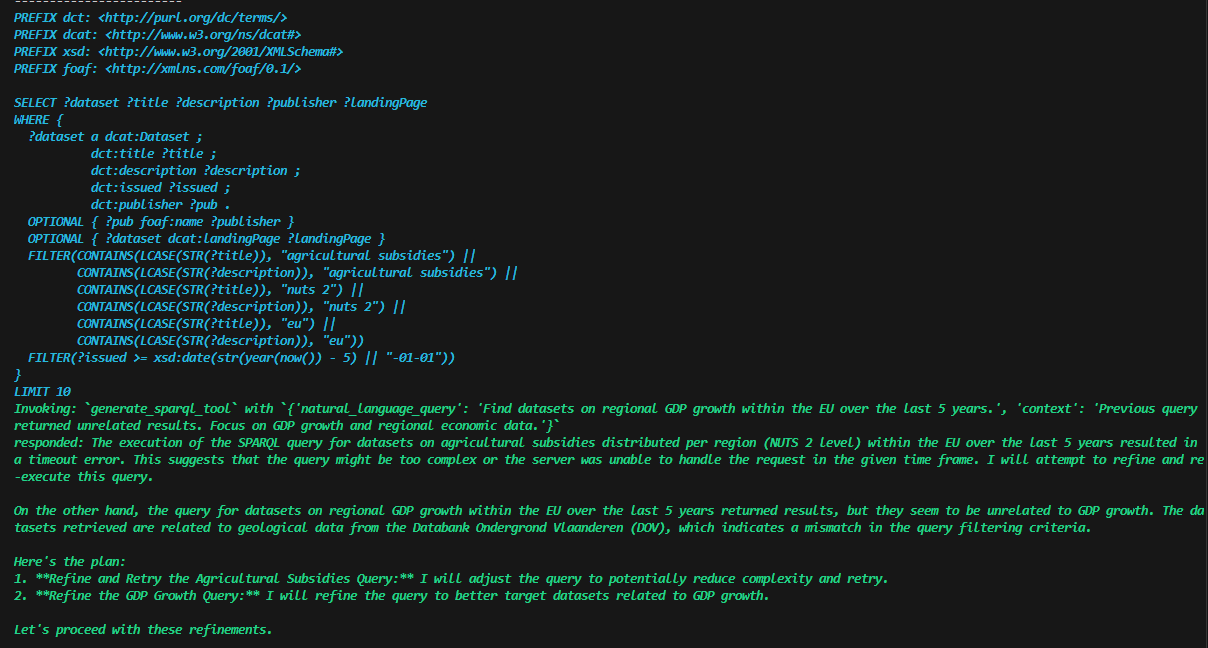
\includegraphics[width=1\textwidth]{figures/izvjestaj_image_68.png}
    \caption{Rukovanje greškama i fallback strategija}
    \label{fig:error_handling}
\end{figure} 
